
%%%%%%%%%%%%%%%%%%%%%%%%%%%%%%%%%%%%%%%%%%%%%%%%%%%%%%%%%%%%
%%%%%%%%%%%%%%%%%%%%%%%%%%%%%%%%%%%%%%%%%%%%%%%%%%%%%%%%%%%%%
%
%  %%%%%%%  %    %  %%%%%%  %%%%%%  %%%%%%%  %%%%%%%  %%%%%
%  %        %    %  %    %  %     %    %     %        %    %
%  %        %    %  %%%%%%  %     %    %     %        %    %
%  %        %%%%%%  %    %  %%%%%%     %     %%%%%    %%%%%
%  %        %    %  %    %  %          %     %        %    %
%  %%%%%%%  %    %  %    %  %          %     %%%%%%%  %     %
%
%%%%%%%%%%%%%%%%%%%%%%%%%%%%%%%%%%%%%%%%%%%%%%%%%%%%%%%%%%%%%
%%%%%%%%%%%%%%%%%%%%%%%%%%%%%%%%%%%%%%%%%%%%%%%%%%%%%%%%%%%%%


\chapter{Cellular Sheaves and Cosheaves}
\label{sec:cell_sheaves}

\begin{quote}
{\em``Sheaf theory is [where] you do topology horizontally and algebra vertically.''}
\begin{flushright} --- attributed to Maurice Auslander by~\cite{gray} \end{flushright}
\end{quote}

We can take it as an experimental observation from Figures \ref{fig:evade_sec_reeb} and \ref{fig:evade_comp} that in certain situations a sheaf or a cosheaf can be described as assigning data directly to the cells of a cell complex. Since cell complexes will be objects of primary importance to us, we review some definitions that may be non-standard.

\section{Cell Complexes and the Face-Relation Poset}

\begin{defn}[Regular Cell Complex~\cite{macpherson-seminar}]\index{regular cell complex}
	A {\bf regular cell complex} $X$ is a space equipped with a partition into pieces $\{X_{\sigma}\}_{\sigma\in P_X}$ such that the following properties are satisfied:
	\begin{enumerate}
		\item {\bf Locally Finite:} Each point $x\in X$ has an open neighborhood $U$ intersecting only finitely many $X_{\sigma}$.
		\item $X_{\sigma}$ is homeomorphic to $\RR^k$ for some $k$ (where $\RR^0$ is one point).
		\item {\bf Axiom of the Frontier}:\footnote{The \textbf{frontier} of a subspace $A$ is the complement of $A$ in its closure, i.e. $\fr(A):=\bar{A}-A$. In some forms this axiom reads: if $X_{\sigma}\neq X_{\tau}$ and $X_{\sigma}\cap\bar{X}_{\tau}\neq\emptyset$ then $X_{\sigma}$ is contained in the frontier of $X_{\tau}$.} If $\Bar{X}_{\tau}\cap X_{\sigma}$ is non-empty, then $X_{\sigma}\subseteq \Bar{X}_{\tau}$. When this occurs we say the pair are \textbf{incident} or that $X_{\sigma}$ is a face of $X_{\tau}$. The face relation makes the indexing set $P_X$ into a poset by declaring $\sigma\leq \tau$.
		\item The pair $X_{\sigma}\subset \Bar{X}_{\sigma}$ is homeomorphic to the pair $\mathrm{int}(B^{k})\subset B^k$, i.e. there is a homeomorphism from the closed ball $\varphi:B^k\to \Bar{X}_{\sigma}$ that sends the interior of the ball to $X_{\sigma}$.
	\end{enumerate}
\end{defn}

\begin{rmk}[Notation]
	Another common way of notating a cell complex is as a pair $(|X|,X)$ where $X$ is the set of cells and $|X|$ is the topological space being partitioned. To each cell $\sigma\in X$ there is a corresponding topological subspace $|\sigma|\subseteq |X|$. Our definition's notation says that $(X,P_X)$ is a cell complex. Our correspondence between cells and subspaces is $\sigma\rightsquigarrow X_{\sigma}$. However, we will have occasion to use both of these notations, and will sometimes use all three symbols $\sigma, |\sigma|$ and $X_{\sigma}$ to mean the same thing.
\end{rmk}

It is true that every regular cell complex can be further decomposed so that the resulting space is the homeomorphic image of a simplicial complex. However, for ease of computations we want to work with a class of spaces more general and natural than regular cell complexes. As such, we work with cell complexes, adopting the same convention as in Allen Shepard's thesis.

\begin{defn}[Cell Complex~\cite{shepard,macpherson-seminar}]\label{defn:face_poset}\index{cell complex}
 A \textbf{cell complex} is a space $X$ with a partition into pieces $\{X_{\sigma}\}$ that satisfies the first three axioms of a regular cell complex. Moreover, we require that when we take the one-point compactification of $X$, then the cells $\{X_{\sigma}\}\cup \{\infty\}$ are the cells of a regular cell complex structure on $X\cup\{\infty\}$.
\end{defn}

\begin{ex}
 The open interval $(0,1)$ decomposed with only one open cell is \emph{not} a cell complex. Its one-point compactification is the circle decomposed with one vertex $\{\infty\}$ and one edge $(0,1)$ whose attaching map is not an embedding, thus contradicting the fourth axiom.
\end{ex}

\begin{defn}[Cell category]\index{category!of a cell complex $\Cell(X)$}
 To a cell complex $(X,\{X_{\sigma}\}_{\sigma\in P_X})$ we can associate a category $\Cell(X;\{X_{\sigma}\})$, which is the indexing poset $P_X$ viewed as a category. This means that there is one object $\sigma$ for each $X_{\sigma}$ and a unique morphism $\sigma\to\tau$ for each incident pair $X_{\sigma}\subseteq \bar{X}_{\tau}$. When there is no risk of confusion, or a cell structure is specified at the beginning, then we will suppress the extra notation and just use $\Cell(X)$ or $X$.
\end{defn}

We now introduce diagrams indexed by the cell category. These were defined in Shepard's 1985 thesis~\cite[p.~6]{shepard}, but were known as ``stacks''\index{stacks} in the first published volume of Zeeman's 1954 thesis~\cite[p.~626]{dihom_1}. However, this term came to be used for an entirely different construction in the landmark paper of Pierre Deligne and David Mumford~\cite{DM-stacks}, which introduced the fundamental concept of algebraic and moduli stacks for algebraic geometry. Zeeman's usage of the term is now extinct, but his work anticipates MacPherson's cellular perverse sheaves (cf. Definition~\ref{defn:cellular_perverse_sheaves}) although MacPherson was unaware~\cite{macpherson} of the content of Zeeman's thesis~\cite{dihom_1,dihom_2,dihom_3}. To keep the presentation simple, we give Shepard's definition and its appropriate dualization.

\begin{defn}[Cellular Sheaves and Cosheaves]\label{defn:cell_sheaves}\index{cellular sheaves and cosheaves}\index{sheaf!cellular}\index{cosheaf!cellular}
	A \textbf{cellular sheaf} $F$ valued in $\dat$ on $X$ is a functor $F:\Cell(X)\to\dat$, i.e. it is 
	\begin{itemize} 
		\item an assignment to each cell $X_{\sigma}$ in $X$ an object $F(\sigma)$,
		\item and to every pair of incident cells $X_{\sigma}\subset \bar{X}_{\tau}$ a \textbf{restriction map}\footnote{Shepard calls these co-restriction maps since they point from faces to co-faces, but we will see they are restriction maps in the Alexandrov topology.} $\rho^F_{\sigma,\tau}:F(\sigma)\to F(\tau)$.
	\end{itemize}
	
	Dually, a \textbf{cellular cosheaf} $\hF$ valued in $\dat$ on $X$ is a functor $\hF:\Cell(X)^{op}\to\dat$, i.e. an assignment of an object $\hF(\sigma)$ for each cell, and an \textbf{extension map} $r_{\sigma,\tau}:\hF(\tau)\to\hF(\sigma)$ for every pair of incident cells $X_{\sigma}\subset\bar{X}_{\tau}$.
\end{defn}

Let us consider a few natural examples.

\begin{ex}[Bott's Torus]\index{cosheaf!cellular!height function on torus}
 The following example was first popularized by Raoul Bott in his book on Morse theory~\cite{macpherson}. Consider the height function on the torus, rotated by $90^{circ}$ so that the real line is underneath the torus, as shown in Figure~\ref{fig:bott_torus}.
\begin{figure}
  \centering
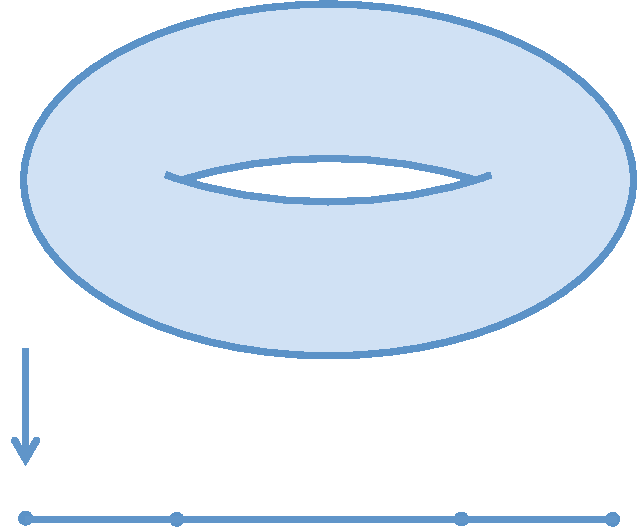
\includegraphics[width=.7\textwidth]{bott_torus_90.pdf}
\caption{Bott's Height Function on the Torus}
\label{fig:bott_torus}
 \end{figure}
 By taking the pre-image of the star of each cell, one obtains a diagram of spaces $\hF:X^{op}\to\Top$. By post-composing this diagram with $H_1(-;k)$, one obtains the cellular cosheaf indicated in Figure~\ref{fig:bott_torus_cosheaf}.
  \begin{figure}[ht]
  \centering
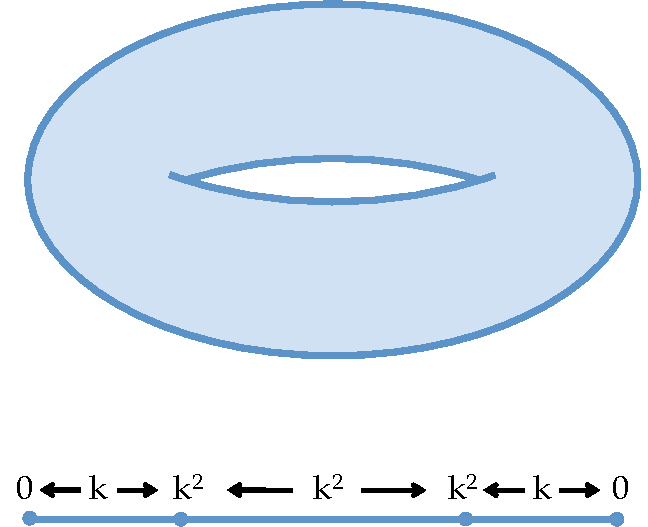
\includegraphics[width=.7\textwidth]{morse_torus_cosheaf.pdf}
\caption{Cellular Cosheaf by Taking $H_1$ of the Star pre-images}
\label{fig:bott_torus_cosheaf}
 \end{figure}
\end{ex}

\begin{ex}[Klein Bottle Revisited]\index{cosheaf!cellular!Klein bottle}
 As seen in Section~\ref{subsec:local_systems}, a Klein bottle can be viewed as a non-trivial $S^1$ bundle over the circle. We've already seen how the this leads to a representation of the fundamental groupoid $\pijuan(S^1)$. We can concoct a cellular cosheaf that describes this bundle in a different way. Let $s$ and $s'$ denote two vertices in a cell decomposition which includes two edges $a$ and $b$, as in Figure~\ref{fig:klein_action}. We can imagine calling the edge $a$ the short edge between $s$ and $s'$ and let $b$ be the long edge. To each cell $\hF$ assigns the homology of the fiber to that cell. The actions are encoded using maps between the cells. This gives us a diagram of vector spaces in the shape of a cell structure on $S^1$:
 \[
  \xymatrix{ & \ar[ld]_{-1} \hF(b) \ar[rd]^1 & \\
  \hF(s) & & \hF(s') \\
  & \hF(b) \ar[ul]^1 \ar[ur]_1 &}
 \]
\end{ex}

\begin{ex}
Let $Y=(0,1)$ be the open unit interval in $\RR$. Denote the inclusion of $Y$ into $\RR$ by $j$. To the constant sheaf on $Y$, written $k_Y$, we can associate two sheaves on $\RR$: $j_*k_Y$ and $j_! k_Y$. To describe these sheaves, we can think cellularly. For the first sheaf $j_*k_Y$ the cellular sheaf is simply the diagram of vector spaces
\[
0 \leftarrow k \rightarrow k \leftarrow k \rightarrow 0.
\]
For $j_!k_Y$ the cellular sheaf is the diagram of vector spaces
\[
0 \leftarrow 0 \rightarrow k \leftarrow 0 \rightarrow 0.
\]
The key difference being that the latter sheaf is zero on the endpoints $\{0\}$ and $\{1\}$. However, one can recover the classical, open set description of the sheaves $j_*k_Y$ and $j_! k_Y$ by considering any ordinary (Hausdorff) open set on the real line and then computing the limit of the diagram that lies over the open set. In Figure \ref{fig:star_shriek} we have drawn the two cellular sheaves of interest and the value of the limit over each open set.
	\begin{figure}
	\centering
	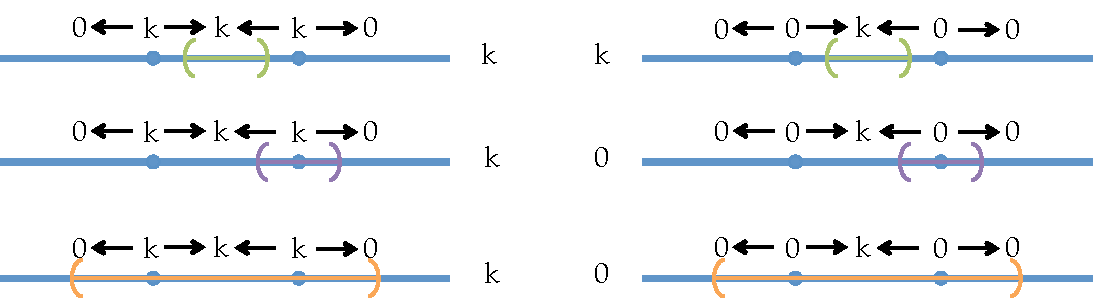
\includegraphics[width=\textwidth]{star_shriek.pdf}
	\caption{Cellular Description of $j_*k_Y$ and $j_!k_Y$ respectively}
	\label{fig:star_shriek}
	\end{figure}
Of course, one can dualize the discussion and consider cosheaves instead and use colimits to get functors from the open set category as defined in Chapter~\ref{sec:abstract_sheaves}. This perspective is developed more fully in Section~\ref{subsec:equivalence_cosheaves}.
\end{ex}

Since functors between categories assemble themselves into a category of their own, we get categories of cellular sheaves and cosheaves.
\begin{defn}\label{defn:cat_cell_sheaves}\index{category!of cellular sheaves $\Shv(X)$, cosheaves $\Coshv(X)$}
 We denote the category of cellular sheaves on $X$ by
\[
 \Shv(X;\dat):=\Fun(\Cell(X),\dat)
\]
and the category of cellular cosheaves by
\[
 \Coshv(X;\dat):=\Fun(\Cell(X)^{op},\dat).
\]
Morphisms are natural transformations of functors. If $\dat=\Vect$, then we will omit the notation after the semicolon and write $\Shv(X)$ and $\Coshv(X)$ instead.
\end{defn}

The notation deliberately coincides with the notation used for categories of sheaves and cosheaves on an arbitrary topological space, i.e. functors out of the open set category that satisfy the appropriate axiom. This conflict will be resolved in Section \ref{subsec:posets} in one way, and in Chapter \ref{subsec:strat} in an entirely different way.

\section{Partially Ordered Sets: Finite Spaces and Functors}
\label{subsec:posets}

Cellular sheaves and cosheaves earn their finiteness by assigning data directly to cells, rather than open sets. This turns out to not be entirely true; Cellular sheaves and cosheaves are simply operating on a different topology than the one we are accustomed to. Partially ordered sets can be endowed with a topology making cellular sheaves and cosheaves into actual sheaves and cosheaves on this topology.  

Here one can illuminate all of the general machinery of classical sheaf theory, but with a combinatorial finiteness that bends the theory to direct computation and understanding. Some of the explicit treatment of sheaves on posets is contained in the clear and concise work of Sefi Ladkani~\cite{sl-dereq}, but we streamline the discussion by using Kan extensions, which clarifies how cosheaves on a poset $X$ differ from sheaves on $X^{op}$.

\subsection{The Alexandrov Topology}
\label{subsubsec:alex}

In this section we introduce a class of non-Hausdorff spaces called \textbf{Alexandrov spaces}. The reader should note that although this topology is non-Hausdorff, it is highly relevant to concepts in algebraic topology. There is a remarkable theorem due to Michael McCord~\cite{mccord-finite} that states that every finite simplicial complex is weakly homotopy equivalence to an Alexandrov space. Thus, if one is interested in the topological properties of simplicial complexes, one should care about (non-Hausdorff) Alexandrov spaces. McCord even gives constructions of classical operations in algebraic topology, including suspension, in the Alexandrov setting. However, our ambitions for this section are far more limited. Let us begin with the necessary definitions.

\begin{defn}\index{preordered set}\index{poset}
	A \textbf{pre-order} consists of a set $P$ and a relation $\leq$ that is reflexive and transitive. A \textbf{poset} is a pre-order where the relation is also anti-symmetric, i.e. $x\leq y$ and $y\leq x$ implies $x=y$. A map $f$ of pre-orders is one that respects $\leq$. That is if $x\leq y$ then $f(x)\leq f(y)$. Pre-orders and order preserving maps form a category $\Preorder$. The collection of all posets form a subcategory of this category.
\end{defn}

Every pre-order can be equipped with a topology. However, it was first defined for finite posets by Pavel Alexandrov~\cite{alex-dr, alex-ct} and the general definition carries his name.

\begin{defn}\index{Alexandrov topology}
	On a pre-order $(P,\leq)$ define the \textbf{Alexandrov topology} to be the topology whose open sets are the sets that satisfy the following property:
	\[
		x\in U \qquad x\leq y \qquad \Rightarrow \qquad y\in U
	\]
	A basis is given by the sets of the form $U_x:=\{y\in P | x\leq y\}$ --- what we will call the \textbf{open star at x}. Similarly, we define the \textbf{closure of x} by $\bar{x}:=\{y\in P | y\leq x\}$. When $P$ is a finite poset, then a basis of closed sets is given by the $\bar{x}$'s.
\end{defn}

Any pre-order $P$ has an associated poset. This poset is gotten by defining an equivalence relation on $P$ via $x\sim y$ if and only if $x\leq y$ and $y\leq x$. One can check that this surjection is order-preserving. This construction defines a right adjoint to the inclusion of posets into pre-orders~\cite{woolf}.

\begin{rmk}[$P$ will mean a poset]
	Although spaces equipped with a pre-order are an interesting class of structures to consider, we will now work exclusively with posets. We do this to prevent closed loops from occurring in chains of related elements, as this would complicate our story.
\end{rmk}

\begin{ex}\label{ex:closed_gen}
	Consider $(\RR,\leq)$ with the usual partial order. The open sets are all those open or half open intervals such that the right-hand endpoint is $+\infty$. Observe that the closed set $(-\infty,0)$ cannot be written as an intersection of closed sets of the form $\bar{t}$. Thus the closures at $t$ do not form a basis.
\end{ex}

The dictionary between cellular complexes and Alexandrov spaces is easily described. First we introduce another definition.

\begin{defn}[Star]\index{star}
	Let $(X,\{X_{\sigma}\})_{\sigma\in P_X}$ be a cell complex. Every cell $X_{\sigma}$ has a \textbf{star}, which is a set that consists of all those cells $X_{\tau}$ such that $X_{\sigma}\leq X_{\tau}$. 
	\[
		\st(X_{\sigma}):=\{X_{\tau}\,|\,X_{\sigma}\leq X_{\tau} \}
	\]
	Since this definition only depends on the incidence relation of cells, we often drop the distinction between $X_{\sigma}$ and its label $\sigma$. Thus the star is also described as a subset of the poset $P_X$ consisting of those labels $\tau$ such that $\sigma\leq\tau$.
\end{defn}

The Alexandrov topology on the indexing poset $P_X$ of a cell complex allows us to define a continuous surjective map that comes from sending each cell $X_{\sigma}$ to its label $\sigma$.
This continuous surjective map gives an alternative way of describing how the Alexandrov topology arises. It is the quotient space where we identify two points $x$ and $y$ if and only if they belong to the same cell.
\[
	\xymatrix{X \ar[d]^{q} \\ P_X:=X/\sim}
\]
The inverse image of the star of $\sigma$ is an open union of cells, which is open. Thus this map is continuous and the topology that makes this map continuous is the Alexandrov topology.

\begin{figure}[ht]
	\centering
	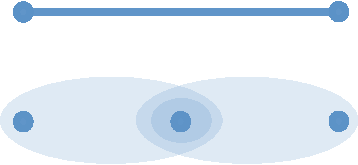
\includegraphics[width=.5\textwidth]{alex_interval.pdf}
	\caption{Alexandrov Space Associated to the Unit Interval}
	\label{fig:alex_interval}
\end{figure}

\begin{ex}[The Interval]\index{Alexandrov topology!unit interval example}
	Suppose $X=[0,1]$ is the unit interval given a cell complex structure with two vertices and one open interval. The face relation poset $P_X$ takes the following form:
	\[
		\xymatrix{ & \bullet & \\ \bullet \ar[ru] & & \bullet \ar[lu]}
	\]
	The Alexandrov topology has basic open sets corresponding to the star of each cell. The stars of the two vertices intersect each other. In Figure \ref{fig:alex_interval}, we have drawn the basic open sets.
\end{ex}

\subsection{Functors on Posets}
\label{subsubsec:fun_kan}
We want to understand how data modeled on posets can be treated as a sheaf or cosheaf on the Alexandrov topology. To do so we use the elegant, but sophisticated, approach of Kan extensions. To motivate this concept we will consider the relationship between a poset and its topology.

Observe that the correspondence between the relation internal to the poset $P$ and the containment relation for the open sets in the Alexandrov topology is order-reversing. Said more succinctly, we have an inclusion functor that is contravariant, i.e.
\[
\iota: P\to \Open(P)^{op} \qquad p \mapsto U_p.
\]
A natural question to ask is 
\begin{quote}\index{Kan extension!motivation}
	``Given a functor $F:P\to\dat$, is there a consistent way of extending $F$ to a functor $R:\Open(P)^{op}\to\dat$?''
\end{quote} 
One can hope to perform this extension since the image of the inclusion $\iota:P\to\Open(P)^{op}$ is a basis for the topology. Consequently, we can express arbitrary open sets as unions (colimits or limits in the opposite category) of basic open sets $\iota(p)=U_p$. A candidate extension would be to define 
\[
F(U):=\varprojlim_{U_p\subset U} F(p)
\] 
or as the colimit of $F$ over $U_p\subset U$. However, we should have some consistency. If one views $U_p=\{p'|p\leq p'\}$ as a subcategory of the category $P$, then it has an initial object $p$ and thus the limit of the diagram $F|_{U_p}$ is $F(p)$, i.e. 
\[
	\varprojlim_{p\leq p'} F(p') \cong F(p).
\]
This guides us to the following possible extension.
% \[
% 	\xymatrix{P \ar[r]^F \ar[d]_{\iota} & \dat \\
% 	\Open(P)^{op} \ar[ur]_-*!/_4pt/{\labelstyle \lim_{U_p\subset U}F(p)=:F(U)} & }
% \]
\[
	\xymatrix{P \ar[r]^F \ar[d]_{\iota} & \dat \\
	\Open(P)^{op} \ar[ur]_-{\varprojlim F(p)} & }
\]
This extension is nice for many reasons. By using limits to define data on larger open sets we have forced the sheaf axiom to hold, so this extension is in fact a sheaf. Moreover it illustrates through example a more general concept, which we now define.

\begin{rmk}[Caveat]
	We will make use of Kan extensions at a few points throughout the paper, but its immediate application is a theorem that says functors out of posets can be identified with sheaves. The proof of this theorem is described casually without the language of Kan extensions in~\cite{sl-dereq}, but adopting this language will be powerful and will make certain categorical properties transparent. 
\end{rmk}

\begin{defn}[Kan Extensions]\index{Kan extension}
	Suppose $\bat,\cat$ and $\dat$ are categories, $F:\bat\to\dat$ and $E:\bat\to\cat$ are functors, then the \textbf{right Kan extension of $F$ along $E$} written $R=\Ran_E F:\cat\to\dat$ is a functor and a natural transformation $\epsilon:RE\to F$ that is universal in the following sense. For every functor $H:\cat\to \dat$ with a natural transformation $\alpha:H\circ E\to F$ there exists a unique natural transformation $\sigma: H\to R$, i.e. $\Nat(H,R)\cong\Nat(H\circ E, F)$.
	\[
		\xymatrix{\bat \ar[r]^F \ar[d]_{E} & \dat \\
		\cat \ar[ur]_-{R=\Ran_E F} & }
	\]
	The \textbf{left Kan extension of F along E} written $L=\Lan_E F:\cat\to\dat$ is a functor with a natural transformation $\eta:F\to L\circ E$ that is universal as well. If $H:\cat\to\dat$ is a functor with a natural transformation $\omega: F\to H\circ E$, then there exists a unique $\tau:L\to H$, i.e. $\Nat(L,H)\cong \Nat(F,H\circ E)$.
	\[
		\xymatrix{\bat \ar[r]^F \ar[d]_{E} & \dat \\
		\cat \ar[ur]_-{L=\Lan_E F} & }
	\]
\end{defn}

\begin{rmk}[Existence of Kan Extensions]
	Kan extensions do not always exist, but we have already alluded to a situation where they do. If $\dat$ has enough limits and colimits, then we can give point-wise formulae for the left and right Kan extensions respectively:
	\[
		\Lan_E F (c):=\varinjlim_{E(b)\to c} F(b) \qquad \Ran_E F (c):=\varprojlim_{c\to E(b)} F(b)
	\]
\end{rmk}

One of the reasons that sheaves and cosheaves on Alexandrov spaces are so well-behaved is that every open set has a finest cover, so in particular, by Corollary \ref{cor:refined_axiom}, we only need to check the (co)sheaf axiom on this cover, and it will be guaranteed for all others. Furthermore, every point in an Alexandrov space has a smallest open neighborhood, and the (co)stalks are just the values on these minimal open sets. This is how we can use Kan extensions to create a dictionary between (co)sheaves on Alexandrov spaces and functors out of posets. 

\begin{thm}\label{thm:posets_sheaves}\index{sheaf!on a poset}\index{cosheaf!on a poset}
	Let $P$ be a poset and $\dat$ a category that is both complete and co-complete. Then the following categories are equivalent
	\[
		\Fun(P,\dat)\cong\Shv(P;\dat) \qquad \Fun(P^{op},\dat)\cong\Coshv(P;\dat)
	\]
\end{thm}
\begin{proof}
	We claim that taking the right Kan extension of $F:P\to\dat$ along the inclusion $\iota:P\to\Open(P)^{op}$ produces a sheaf. Suppose $U$ is an open set in the Alexandrov topology, i.e. one for which $p\in U$ and $p\leq p' \Rightarrow p'\in U$. It is true that every open set can be expressed as a union $U=\cup_{p\in U} U_p$ and thus the finest possible cover is $\{U_p\}_{p\in U}$. The right Kan extension then defines $F(U):=F[\{U_p\}_{p\in U}]$ so the sheaf axiom holds for that cover, but by Corollary \ref{cor:refined_axiom}, this means that $F$ is a sheaf. To go from a sheaf to the diagram, one simply takes stalks at every point. Since the smallest neighborhood containing $p$ is $U_p$, we get that $F_p=F(U_p)=F(p)$. 
	
	The dual argument for cosheaves is completely analogous: we take the left Kan extension of $\hF:P^{op}\to\dat$ along the inclusion $\iota:P^{op}\to \Open(P)$ to get a cosheaf. Taking costalks returns a diagram from a cosheaf.
\end{proof}

\begin{rmk}[Stalks and Costalks on Posets]
	To elaborate on the proof, let us compute some invariants. Recall that the stalk and costalk at a point $p\in P$ for a sheaf and cosheaf respectively is described via the use of filtered colimits and limits.
	\[
	F_p:=\varinjlim_{U\ni p} F(U) \qquad \mathrm{and} \qquad \hF_p:=\varprojlim_{U\ni p} \hF(U)
	\]
	In both cases when $P$ is a poset with the Alexandrov topology there is a smallest open set containing $p$, namely $U_p=\{q|p\leq q\}$, so $F_p\cong F(U_p)=F(p)$ and $\hF_p=\hF(U_p)=\hF(p)$.
\end{rmk}

\begin{defn}[Sections]\label{defn:sections}\index{sheaf!sections over a poset}\index{cosheaf!sections over a poset}
	Let $(P,\leq)$ be a poset and $F:P\to\dat$ a sheaf and $\hF:P^{op}\to\dat$. let $Z\subset P$ be any subset. We define the \textbf{sections over $Z$} to be
	\[
		\Gamma(Z;F):=\varprojlim F|_Z \qquad \mathrm{and} \qquad \varinjlim \hF|_Z=:\Gamma(Z;\hF).
	\]
	When $Z=P$, we call these \textbf{global sections}. Note that $\Gamma(Z;-)$ is context dependent: different definitions are used pending whether a sheaf or cosheaf is used.
\end{defn}

The above theorem provides the simplest explanation of why cellular sheaves and cosheaves deserve to be called sheaves and cosheaves. When Theorem \ref{thm:posets_sheaves} is specialized to the face relation poset $P_X$ of a cell complex, also called the cell category $P_X=\Cell(X)$ in Definition \ref{defn:face_poset}, we get that the category of sheaves in Definition \ref{defn:cat_cell_sheaves}. We summarize these observations in the following corollary. 

\begin{cor}
	Let $(X,P_X)$ be a cell complex. A \textbf{cellular sheaf on $X$} is a sheaf on $P_X$ equipped with the Alexandrov topology. Such a sheaf is uniquely determined by a functor $F:P_X\to\dat$. A \textbf{cellular cosheaf on $X$} is a cosheaf on $P_X$ with the Alexandrov topology. Such a cosheaf is uniquely determined by a functor $\hF:P_X^{op}\to\dat$.
\end{cor}

To close, we point out one of the symmetries that Alexandrov spaces possess.

\begin{clm}
	In the Alexandrov topology, arbitrary intersections of open sets are open and arbitrary unions of closed sets are closed. Thus, every Alexandrov space possesses a dual topology by exchanging open sets with closed sets.
\end{clm}
\index{cosheaf!on closed sets}\index{sheaf!on closed sets}
This observation would have pleased Leray. It demonstrates that one can also think of a functor $F:P\to\dat$ on a poset as either a sheaf or as a ``cosheaf on closed sets.'' What distinguishes these two though is whether we use limits or colimits to extend to larger sets. We will consider this perspective in greater detail in Section \ref{subsubsec:closed_push}.

